Despite simplicity of electric nature, the electricity sector is complex in operation and regulation.
Nonetheless, when considering power demand, security to transport and to generate energy, fair investments to keep all the infrastructure working, standards to better integrate markets and industries, laws to guide and protect users and so on, the sector starts to take its format.
The number of consumers to count in is not just one more specification, but the main reason why all this complexity exist.

% Para sanar as dúvidas (definições) -- 06/07/18
% http://www2.aneel.gov.br/cedoc/res2002102.pdf
% http://www2.aneel.gov.br/cedoc/ren2004109.pdf
% Glossário de Termos / Interpretações e Relação de Acrônimos (drive) -- 07/07/18

Generally, the electric power infrastructure is presented as the electricity sector behavior.
However, this approach results in a lack of knowledge on regulations and energy trade.
The former comprises the energy flow through generation to consumption spots, its equipment and humans-work, possessing the same structure anywhere.
Whilst the latter encompasses the economic, regulatory and political subjects, as shown on \autoref{fig:sector}.
The countries have similar approaches to manage electricity, but do so accordingly with its personal scenario.

\begin{figure}[h!t]{\textwidth}
	\centering
    \caption{Slight difference between electricity sector concepts.} \label{fig:sector}
    
    \tikzstyle{arrow} = [thick,->,>=stealth, line width=1pt]
    \tikzstyle{drew} = [draw,fill=white,rounded corners=0.1cm]
    
    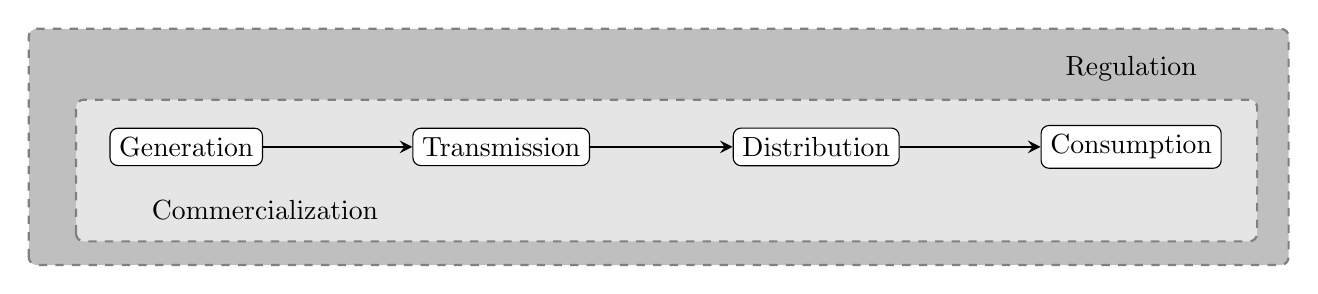
\begin{tikzpicture}
        % place dimensions
        \draw[gray,thick,dashed,fill=gray!50,rounded corners=0.1cm] (-2,-1.5) rectangle (14,1.5);
        \draw[gray,thick,dashed,fill=gray!20,rounded corners=0.1cm] (-1.4,-1.2) rectangle (13.6,0.6);
        
        % place nodes
        \node[drew] at (0, 0)		(g) {Generation};
        \node[drew] at (4, 0)		(t) {Transmission};
        \node[drew] at (8, 0)		(d) {Distribution};
		\node[drew] at (12, 0)		(c) {Consumption};
        \node		at (1, -0.8)	(o) {Commercialization};
        \node		at (12, 1)		(r) {Regulation};

        % draw connections
        \draw[arrow] (g) -- (t);
        \draw[arrow] (t) -- (d);
        \draw[arrow] (d) -- (c);
    \end{tikzpicture}
    
  	\legend{While electric power basic infrastructure is on white boxes,
    electricity sector pattern involves greater integrations as shown by gray boxes.
    The presence and relationships of agents on each segment is indicated as well.}
    \source{Author.}
\end{figure}

\Autoref{fig:sector} captures the stakeholders on the sector and their common relationship, but their classifications varies by means of their roles.
They are designated as agents in Brazil with an exception for the consumers, that despite always represent the end of electricity chain, they might be placed after the distributer or transmitter agents.
% that are classified by power consumption based on economies of scale, that is, tariffs are inversely proportional by power demand levels~[ref]. (xu2017 fala isso)
In addition, each agent has to fit in its corresponding segment regulation, i.e.,
any transmitter agent has to agree with the transmission segment procedure,
any generator, with the generation segment one, and so forth.
The exceptions are, again, the consumers, in particular, because they have different rules to conform to, based on their energy needs and relational segment.

In this way, the consumers have a broad classification, that's why they are not fully represented by one single agent or fit in a solely segment, but they can be essentially split into two groups, namely
\begin{enumerate*}[label={{(\roman*)}},itemjoin={{; }},itemjoin*={{; and }}]
    \item regulated (or captive) consumers, these ones fed by distribution utilities with fixed monthly tariffs
    \item free consumers, which are fed by whoever has the capacity to feed its power needs by means of a bilateral agreement
\end{enumerate*}
~\cite{agentes,lud2007}.
The former, which is our target group, are subclassified as residential, industrial, commercial, rural and public consumers~\cite{tarifas}.

The possibility of consumers participation on the distribution grid as generator has incentivize the ``segment'' of \gls{gd}.
The latter is defined in Brazil into two categories -- micro or mini -- upon from its limits of the installed power source,
the consumer's role switch to the prosumer, a producer and consumer of electricity.
Together with the increase of \gls{ict} management on the electricity sector, which has been evolving towards a smart grid,
the \gls{gd} is one of the predictions with more ruptures in the sector, given its impact on power infrastructure, and business behavior.

The following paragraphs present an overview of the Brazilian electricity sector, emphasizing the \gls{gd} context and some other aspects of the sector that can be useful to support the development of the proposed application.

\section{The electricity sector in Brazil: a DG approach~\label{sec:brazil-sector}}

Usually, Brazilians can supply their power demands by renewable energy or by natural gas cogeneration system and send their surplus power back to local distribution grid as power credits for later consumption.
This power source alternative is known as \gls{gd} and it is categorized as micro/mini grid accordingly with technical requirements of power generation capacity.
Besides individual benefits, the whole sector can get positive impacts, such as ``postponement of investments in expansion of transmission and distribution systems, low environmental impact, reduction in network loading, minimization of losses and diversification of the energy matrix''.
Further, the legislation keeps on improvement to meet stakeholders needs and to admit innovation on the sector~\cite{GD}.

Despite appealing invitation to join in this manner of power generation, the cost feasibility to allow its expansion is still high for most of citizens, even with recently government tax incentives~\cite{ideal2017} and improvements on technical specifications (\gls{aneel} office Number 720, March 25th, 2014).
For instance, the \gls{gd} had no significant involvement on national power consumption for residential and commercial classes,
\textcolor{red}{which together represented only $3 GWh$ on 2014, but it was expected one-third (? 0,33\% ?) rise up for its portion for each class, which should represent a sum of $1072 GWh$ ten years ahead, on 2023~\cite{epe2014}.}
% Nowadays, in mid 2018, its has reached almost $x GWh$ for both classes and counting~\cite{GD}. % Só tem potência... :/ Ver o relatório de 2018 do Instituto Ideal lançado hj (04/05/18)

Moreover, the consequences of \gls{der} on system reliability are always on focus because its particular characteristic of generation within a period implies into new challenges such as:
load forecasting;
interference on voltage levels;
guidances to handle with the amount of information;
the need of specialized command and control~\cite{debra2017};
optimization of generation in small self-sustaining communities with use of Electric Vehicles and network balancing~\cite{Coelho2016730} in order to mitigate power quality problems;
and provide active power as demanded by loads~\cite{thomas2017}.

In addition to these aforementioned mentioned points, economic issues can arise such as cross-subsidies~\cite{iea2011,epe2014},
in which upper tariffs are needed to compensate utility revenue diminished by the presence of \gls{gd} on the grid.
In summary, it means that general people subsidy the ones benefiting with \gls{gd} installations.
Further, it is considered a business model disruption that can threaten the economic equilibrium of the power services~\cite{gianelloni2017}.

Consequently, we are still embraced by big power plants instead of \gls{gd}.
For instance, Brazilian governement is still investing in the construction of large scale projects, such as Belo Monte hydropower plant.
The Brazilian electrical matrix is basically a renewable one in comparison with world's electrical matrix.
The former has mainly hydroelectric plants supporting national power demand.
In several nations around the globe the main energy source is based on fossil fuels such as coal, oil and natural gas in thermoelectric plants~\cite{abcdenergia}.
Nowadays, Brazil has in operation almost $160GW$ of installed power when considering the sum of hydroelectric plants of any size, which represents more than 60\% of the total power consumption, while thermoelectric plants accounting for 26\%~\cite{BIG2}.
It supplies electricity for each $209$ million of inhabitants~\cite{ibge-pop}.
Whereas only $43.934$ consumer units take advantage of \gls{gd} totalizing a installed power capacity of almost $374MW$,
with photovoltaic solar power constituting 77\% of it~\cite{BIG2}.

Considering that Brazil is a country with continental dimensions, and aware of electricity impact on national economic growth, the Government has particular directives to manage and operate the power flow throughout each place.
One of them is maintaining the power network as a unit, known as \gls{sin}, where a set of installations and types of equipment are electrically connected across regions, these ones grouped in four subsystems, to allow power supply.~\cite{sin}.

Furthermore, on the current fundamentals to manage the whole electricity sector there are three principles:
\begin{enumerate*}[label={{(\roman*)}},itemjoin={{; }},itemjoin*={{; and }}]
	\item seek the lowest feasible tariff and price
    \item ensure security on electricity supply -- by guaranteeing enough generation on reducing high risks notion in this sector and allowing fair return to investors
    \item promote social integration -- connecting isolated areas to the \gls{sin} or, meanwhile, through programs to provide off-grid energy for citizens
\end{enumerate*}%
~\cite{modeloBR,lud2007}.

The regulatory structure that supports this sector is directed by the \textbf{\gls{mme}}, which, in conjunction with other administrations, aims to better serve electricity demand by planning power generation expansion and attracting required private capital investments.
In short, the supporting administrative bodies and their assignments are
\begin{descriptive}
	\item[\gls{aneel}] responsible for regulating and carrying out long-term investments in the sector, such as develop tariff calculation methodologies for the various segments% ``The agencies also oversee the market, bearing in mind the principals of free market enterprise, consumers' protection, free entry and competition.''
    \item[\gls{ccee}] responsible for energy trade subjects, such as managing ``long-term bilateral contracts among generators and distributions utilities and the settlement of contractual differences for all market agents''
    \item[\gls{cmse}] which permanently evaluate the security of electricity supply
    \item[\gls{epe}] responsible for planning the long-term electricity sector (10- and 20-year expansion studies)
    \item[\gls{ons}] responsible for operational control and management of the generation and transmission facilities at \gls{sin}
\end{descriptive}%
~\cite{modeloBR,tarifas,lud2007}.

Additionally, the sector operates by two trading markets (supply markets) that comprises the
\begin{itemize*}[font=\bfseries]
	\item[\gls{acr}] where regulated (or captive) consumers are supplied by distribution utilities under a supervised energy trade managed by \gls{aneel}; and the
    \item[\gls{acl}] where free consumers must negotiate electricity price directly with supply agents (generating or market agents) through freely bilateral contracts signed at \gls{ccee}
\end{itemize*}%
~\cite{market,lud2007}.
Although, \gls{acl} could look more tempting,
the consumer role is specified by technical regulations and power conditions management, which limits the transition between one market to another, but guarantees a well planning and operation of the grid.

The prevalent trade model emphasizes actions towards customer-centered policies, mainly at the \gls{acr} context.
In addition, ``to avoid the charge of unjustified hidden costs by distribution companies for energy supplied to captive consumers''~\cite{lud2007},
the purchase of power by distribution agents must be through auctions carried out by \gls{ccee}, on behalf of \gls{aneel},
which, in turn, uses the criterion of lowest price of generation in order to reduce the acquisition cost of electricity to be passed on~\cite{modeloBR}.

\subsection*{Finance matters}

The electricity tariff aims to ensure sufficient revenue for distribution utilities
to cover operating costs,
to remunerate necessary investments for the expansion of power capacity,
to guarantee quality services,
and to create incentives for efficiency~\cite{price,tarifas}. % ANEEL [2017b] - [ANEEL, 2016b].

As previously said, in the \gls{acr} market -- which \gls{gd} stands for -- customers are still classified by classes such as residential, industrial, commercial, rural and public energy.
% A classification that does not define customer power needs, but its sector...?
But, whilst all of them are captive consumers and have the lowest possible tariff, % guarantee by \gls{aneel}
they differ in terms of tariff granularity by power consuming and demand,
in which small power consumers pay only for the former, % grupo B
while greater ones pay for both, beyond the condition to opt for tariff diversification by time frames. % grupo A
% A measurement that is expected to change over time, meanwhile, the current actions are described on the following subsection.
% REESCREVER!!!
% Demanda - é a potência média verificada em intervalos de 15 min.

The electricity tariff is charged by energy consumed (R\$/kWh) and availability -- 24 hours a day throughout the whole year. % [ABRADEE, 2017a].
It is strictly regulated by \gls{aneel}, because it is an essential good,
and it is composed of costs incurred from generation and transmission segments,
which indeed is the remarkable component that represents more than half of the final value~\cite{price}.

The cost of generation consists of each power plant availability present in the \gls{sin}~\cite{fontes}, and
forecasting analysis of the hydroelectric generation feasibility at the present time and in the future by periods and subsystems~\cite{arteiro}. %[de Oliveira, 2006]
This calculation made by \gls{ons} also consider the power transmission capacity between each subsystem and the energy availability in each time frame for defining the best price~\cite{fontes}.

Thereby, the final generation cost definition stands between its lowest level, just given by hydroelectric costs, to the highest level, just operated by thermoelectric ones~\cite{arteiro}.
The former is not only due to the quantity offered, but mainly due to the efficiency when compared to the cost of installation and the ``fuel'' used~\cite{fontes}. % [CCEE, 2017c].
Nonetheless, the latter is very worth, because they can be dispatched anytime without restrictions imposed by water limits.
Notably, the former is preferred to keep grid powered on, whilst the latter is used to keep system working well during power peaks.
The optimization of these costs guarantees the modality of tariffs in all subsystems of the \gls{sin} and uninterrupted electricity for all Brazilian citizens~\cite{arteiro}.

Although the above methodology is a public statement,
it has started to be clearly available to the population only in 2015~\cite{bandeiras},
with the value of electricity being detailed on the energy bill.
In other words, since that year the monthly cost of power generation has started to be visually discriminate on the energy bill,
by showing a flag that can have three different colours -- green, yellow or red -- to indicate generation threshold.
A determination that aims to educate residential consumers % pois bandeiras tarifárias SÓ SE APLICAM a classe RESIDENCIAL e nosso foco é justamente esta classe!
about power generation condition on the country, i.e.,
the Tariff Flags System depicts unfavourable situations in the \gls{sin},
where there is a need for a thermoelectric generation to compensate (or to ensure future) hydroelectric generation~\cite{bandeiras}.% [ANEEL, 2017c]

Another measurement recently announced to be extended to the residential class is tariff diversification according to the day and time of power consumption,
in other words, during working days the period of high demand of power, known as peak time, has higher tariff, otherwise the value is lower than the conventional tariff
% Called White Tariff, it is favorable for consumers that decrease consumption of energy when it is more required
~\cite{tarifa_branca}. % [ANEEL, 2017d]

% \subsection{A GD como alternativa aos custos de geração de EE}

% [linkar melhor estes parágrafos -- ending]

As it can be seen, the \gls{gd} can come to the rescue of diverse price options for power generation.
Faced with range of possibilities
from different types of power source (single-wind turbines, biomass generators, solar power and so on),
to equipment technology,
and to local of installation (rural or urban),
consumers may benefit from an alternative personal tariff based on pros and cons of the project financing and on the existence of other consumers to venture share~\cite{GD}.% [ANEEL, 2016c].

% \subsection*{The DG structure}

% The prosumers are grouped by the Brazilian regulation into four categories,
% but they can be divided into two main groups based on their generation management,
% one that is for self-consumption, and another for shareable one.
% The former is for individual use.
% The \gls{gd} may be on the same local of power consumption or
% in another place -- namely \emph{remote self-consumption} -- whereas the power and consumption units must be inside the same distribution utility coverage area.
% The latter refers to sharing generation between customers,
% either they are from a condominium -- known as \emph{enterprises of multiple consumer units} -- or
% from a consortium or a cooperative -- known as a \emph{shareable generation}.
% Again, the customers' units must situate inside the same distribution utility coverage area.
% Furthermore, at the shareable consumption group, the principles about how the generation will be split are up to their members' guidelines~\cite{GD}.

% Nonetheless, independently of group type,
% the surplus energy generated can be ``stored'' on the distribution grid by no additional cost in order to be consumed later by the respective consumer, a measure known, in Brazil, as the Electricity Compensation System~\cite{FAQ}. % [ANEEL, 2016a]
% This ``energy credit'' can only be used for personal purposes, i.e., it can not be transferred for anyone, even if part of a shareable consumption group,
% however, the group's quota can do so based on members' guidelines.

% --------------------------------------------------------------------------------
% However, pricing the cost of electricity provided by the consumer is an arduous task,
% because each individual has a different cost reference.
% Even with all the advantages of having GD,
% there is an unstable point in this configuration,
% the discrepancy in the commercialization of energy,
% since the differences are settled in kWh,
% considering the different bases of calculation of the cost of generation by the distributor and the system of GD.